\documentclass[12pt,conference]{ieeeconf}
\bibliographystyle{ieeetr}
\usepackage{graphicx}
\usepackage{float}
\graphicspath{{/}}
\begin{document}
\title{Case Study: Data parallelization using Pytorch}
\author{Brian Rodriguez, University of Utah}
\maketitle

\section{INTRODUCTION}
	With recent advancements in Machine and Deep Learning, developers have a tendency to use more computing power than necessary. Spreading their data and models across several GPUs is not always the best option when training neural networks. When a developer spreads their model across more than 3 GPUs its not uncommon to see a slow down and also accuracy loss. This case study aims to bring light to the fact that more does not always mean better.
	
\section{PYTORCH}
	Pytorch is an amazing open source deep learning library for python. It allows a developer to create neural networks with ease. I had an option to choose between Pytorch and Caffe2 but I chose to stick with Pytorch since developing neural networks is far more trivial than Caffe2. Also, a huge part of a framework is documentation and from my experience Caffe2 is by far the worst documented deep learning framework I have used. Its safe to say that Pytorch trumps a lot of the deep learning frameworks and is the most intuitive. Integrating data parallel constructs and multiple GPUs is a breeze. It also became easier to train across multiple GPUs with the new 0.4.0 Pytorch release. Now only minor tweaks to existing code can allow for training on a CPU or GPUs.
		
\subsection{DATA PARALLEL CONSTRUCTS IN PYTORCH}
	Pytorch offers many data parallel constructs that make it easier for a developer to train across multiple GPUs and not have to worry about a message passing interface. Depending on the type of training a developer plans on doing, whether that is training on a machine or across node clusters there are constructs for both cases. The construct I used was training on a single machine with multiple GPU cards. The data parallel construct essentially distributes the data across all of the GPUs so that operations can be done on the neural network accordingly. The distributed training construct is similar to the data parallel construct but requires an extra level of abstraction. It requires the implementation of message passing operations similar to those in MPI and gloo. There is a tutorial on how to navigate this interface but for the purpose of this case study, it was not required.
	 
\section{VGG19}
	For the purpose of this case study, I chose to implement VGG19 \cite{VGG19}. I had an abundant amount of options and wanted to implement a deep enough neural network to show the side affects of parallelizing data. VGG19 is 19 convolutional layers coupled with ReLU activations, contains 4 maxpooling layers, 3 fully connected layers and 1 soft-max layer. Another network I took into consideration was InceptionV4 \cite{IN4} but this network contains 192 layers and would have caused even more problems that I discuss in more detail in further sections.
	
	The dataset used in these experiments was CIFAR10 which contains 10 classes and 6000 images per class of size 32x32. A total of 50,000 training images and 10,000 test images. The images are resized to 224x224 to fit VGG19's structure, randomly shuffled, and normalized.
	
\begin{figure*}
\begin{center}
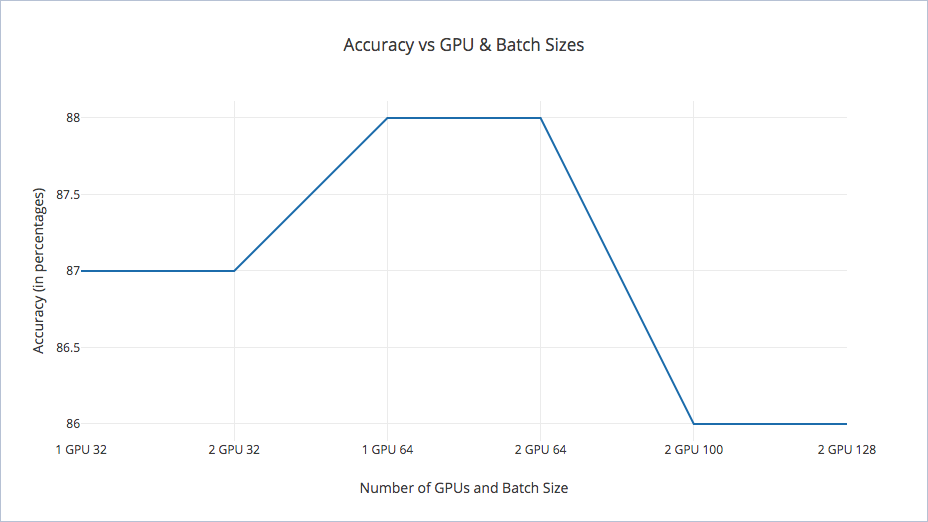
\includegraphics[width=2.0\columnwidth]{Accuracy}
\end{center}
	\caption{\textbf{Shows the difference in accuracy between GPUs and their respective batch sizes.}}
\label{fig:ACC}
\end{figure*}
	
\section{RESULTS}
	Training neural networks of this size takes a considerable amount of time. With many faulty test runs, the results that I have gathered are still not concrete to prove that this case study is correct. Due to problems discussed in the next section, I was unable to gather tests with 3 GPUs. Also, there are gaps between batch sizes between 1 and 2 GPUs. When using only a singular GPU, if the batch size is large enough then it reports an out of memory error. On 2 GPUs, this is not the case since the batch size is split in half and each GPU works on its respective half.
	
	When comparing the training time between 1 and 2 GPUs, it is easy to see that as the batch size increases the time spent training decreases. Except for the case of a batch size of 32. As the batch size gets smaller, its much more efficient to just use a singular GPU. The time increases since there is more overhead communication that must be done between GPUs. In the case of a batch size of 64, the time to train is almost halved. Normally, it is good practice to increase the batch size in powers of 2. When the batch size is 100 in this case the time to train increases, which I thought was odd but for this reason it may or may not show that increasing the batch size in powers of 2 is good practice.
	
	Comparing the accuracy measurements between 1 and 2 GPUs actually shows that the accuracy does not change as you increase the number of GPUs. Although, this is not an exhaustive study of this problem. The weights were initialized in the same fashion, meaning that no matter how many times I increase the number of GPUs or batch sizes the calculations should yield similar results. However, as the batch size increases the loss of the entire neural network changes each iteration. The loss is used to compute the gradients of the network and used to update the weights respectively. This would explain the difference in accuracy as the batch size increases.
	
	From the results, it seems that a batch size of 64 is suitable enough to yield the best results in my case, with respect to time taken to train and overall accuracy. Although, the purpose of this case study was not to find the most efficient batch size when using GPUs, it is still a great observation. For reasons discussed in the next section, I was not able to do a full-fledged exhaustive study. 
	
\begin{figure*}
\begin{center}
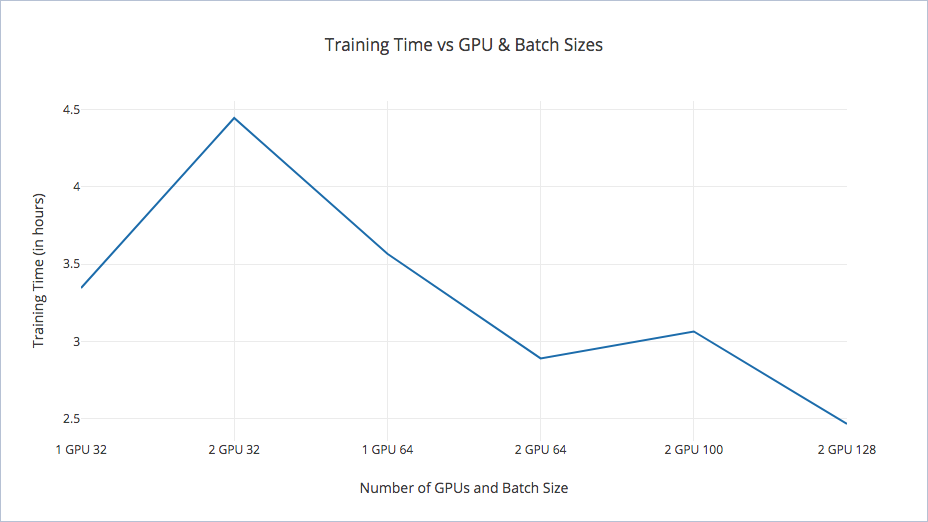
\includegraphics[width=2.0\columnwidth]{TrainingTime}
\end{center}
	\caption{\textbf{Shows the time elapsed between GPUs and their respective batch sizes.}}
\label{fig:TT}
\end{figure*}

\section{DEVELOPMENT SETBACKS}
	During development, there were many hurdles that halted my development completely. The initial problem that I ran into was the neural network I created would not learn, the loss value of the network would plateaued at around 2.1. Meaning the the loss was not being backpropagated through the neural network and thus not learning. It turns out, Pytorch requires that every variable created must have a flag that requires a gradient to be propagated through it. Meaning, if a variable does not have this flag then backpropagation will not perform an update to the variable. When creating VGG19, I left out these flags and thus the network did not learn.
	
	Training VGG19 across multiple GPUs is a different ball game than simply training on a CPU or a single GPU. There were many tests I was not able to conduct because training across multiple GPUs caused too many issues. The initial tests of a singular GPU did not bode so well with a large batch size. This is to be expected since there is only so much memory on a GPU. However, I did not expect to run into cuda out of memory errors when training across multiple GPUs. Even with a small batch size of 12, the training came to a halt. It turns out, Pytorch has some sort of data imbalancing issue when training across multiple GPUs. When a forward pass of the network is done and the loss is calculated, the underlying framework then does a backward pass across the entire network. After, the framework does a gather operation and shifts all of the updated matrices to a singular GPU. This gather operation is the bottleneck that causes the cuda out of memory errors. Since each GPU has its own copy of the network then when the gather operation is called the entire network and its respective gradient updates are shifted onto a singular GPU. Pytorch's variables track history and have their own underlying graphs associated with them. These underlying graphs are tremendously large and contain a history of all of the previous operations that were done on a single variable Since gradients are the final operation in a graph, the graph tends to be large; containing the entirety of the network and its operations. When this gradient variable is shifted onto a singular GPU along with the other gradients calculated on the other GPUs then one can see how the GPU runs out of memory.
	
	I still have yet to solve this problem and is an ongoing development for me. Currently, I have this strange suspicion that it is due to the CHPC cluster. It seems to me that this operation should be gathered on the CPU and not a GPU since a CPU tends to have more memory available. When gathering allocation time from the CHPC cluster, it only gives me access to the GPUs and very minimal CPU memory. Normally, I feel like this sort of out of memory error should not be happening if I had a machine with the required resources. I hope soon I am able to solve this problem as multiple GPU training is something I plan on doing in future research developments.	
	
\section{RELATED WORK}
	Initially, I chose to implement a Virtualized Deep Neural Network \cite{VDNN}. I was excited about this project since neural networks these days tend to be large in size and require a lot of RAM. The vDNN aims to combat this problem by prefetching various layers and releasing the memory these layers occupy when needed. Unfortunately, after further research, I came to the conclusion that this project would require more time and effort. I found that implementing the vDNN is close to impossible when using a deep learning framework. I looked into using caffe2, pytorch and even tensorflow but neither of the three allow the user to prefetch layers and release memory. The only memory optimizations the frameworks allowed a user to tinker with were the different caching styles but even this required the user to rebuild the code from source.
	
	I spent the better half of two weeks researching different ways I could implement the vDNN; I came to the conclusion that I'd have to manually create the machine learning primitives and implement the vDNN in C++. This would require months of work to accomplish and would be better suited for a personal project. Vinu suggested another great idea of doing a similar project but instead it would be a case study on data parallelization using Pytorch.

\section{CONCLUSION}
	Unfortunately, I was not able to gather concrete evidence on whether spreading a model and its respective data across multiple GPUs causes a slowdown and or accuracy loss. The hurdles I faced became out of my control and as my ongoing development continues, I still want to solve the out of memory problem and hope in the future I can finish this case study.

\bibliography{biblio}

\end{document}